\documentclass[tikz]{standalone}
\usepackage{tikz}
\usetikzlibrary{%
    patterns, plotmarks, backgrounds, shapes, arrows, calc, trees, positioning,
    chains, shapes.geometric, decorations.pathreplacing,intersections,
    decorations.pathmorphing, shapes.arrows, decorations.markings, quotes,
    arrows.meta, spy, fit, matrix, math,
}
\usepackage{amsmath,amsthm,bm}

% General image and colour support
\usepackage{graphicx}
\usepackage{xcolor}

% Captions and subcaptions
\usepackage{caption}
\usepackage[labelformat=parens]{subcaption}

% Define colours
\definecolor{cred}{HTML}{ED1C24}
\definecolor{cgrey}{HTML}{7F7F7F}
\definecolor{cblue}{HTML}{00A2E8}
\definecolor{cgreen}{HTML}{22B14C}
\definecolor{cyellow}{HTML}{FFF200}
\definecolor{corange}{HTML}{EA7904}
\definecolor{cpurple}{HTML}{9100FC}

\definecolor{cyto}{HTML}{1F77B4}
\definecolor{mito}{HTML}{2CA02C}
\definecolor{else}{HTML}{FF7F0D}

\definecolor{efm1}{HTML}{017EC3}
\definecolor{efm2}{HTML}{F31E26}
\definecolor{efm3}{HTML}{019E5E}
\definecolor{efm4}{HTML}{FBA61D}
\definecolor{efm5}{HTML}{916237}

% Define main node types
\tikzstyle{node} = [%
    circle,
    draw=black,
    minimum height=0.5cm,
    line width=1.0pt,
    align=center,
    fill=cgrey,
    fill opacity=1.0,
    text opacity=1.0,
    text centered,
    text=black,
    inner sep=1.0pt,
    font=\normalsize
]
\tikzstyle{nodeT1} = [%
    rectangle,
    rounded corners=5pt,
    fill=white,
    draw=black,
    minimum width=1.5cm,
    minimum height=0.8cm,
    line width=1.0pt,
    align=center,
    fill opacity=1.0,
    text opacity=1.0,
    text centered,
    text=black,
    inner sep=3.0pt,
    font=\normalsize
]
\tikzstyle{nodeT2} = [%
    rectangle,
    rounded corners=5pt,
    fill=white,
    draw=black,
    minimum height=1.5cm,
    minimum width=0.8cm,
    line width=1.0pt,
    align=center,
    fill opacity=1.0,
    text opacity=1.0,
    text centered,
    text=black,
    inner sep=3.0pt,
    font=\normalsize,
]

\tikzset{%
    position/.style args={#1:#2 from #3}{%
        at=(#3.#1), anchor=#1+180, shift=(#1:#2)
    },
    double -latex/.style args={#1 colored by #2 and #3}{%
        -latex,line width=#1,#2,
        postaction={draw,-latex,#3,line width=(#1)/3,shorten <=(#1)/4,shorten >=4.5*(#1)/3},
    },
    double -latex2/.style args={#1 colored by #2 and #3}{%
        latex-latex,line width=#1,#2,
        postaction={draw,latex-latex,#3,line width=(#1)/3,shorten <=4.5*(#1)/3,shorten >=4.5*(#1)/3},
    },
    double -line/.style args={#1 colored by #2 and #3}{%
        -,line width=#1,#2,
        postaction={draw,-,#3,line width=(#1)/3,shorten <=4.5*(#1)/3,shorten >=4.5*(#1)/3},
    }
}

\usepackage{amsmath}
\renewcommand{\familydefault}{\sfdefault}

\begin{document}

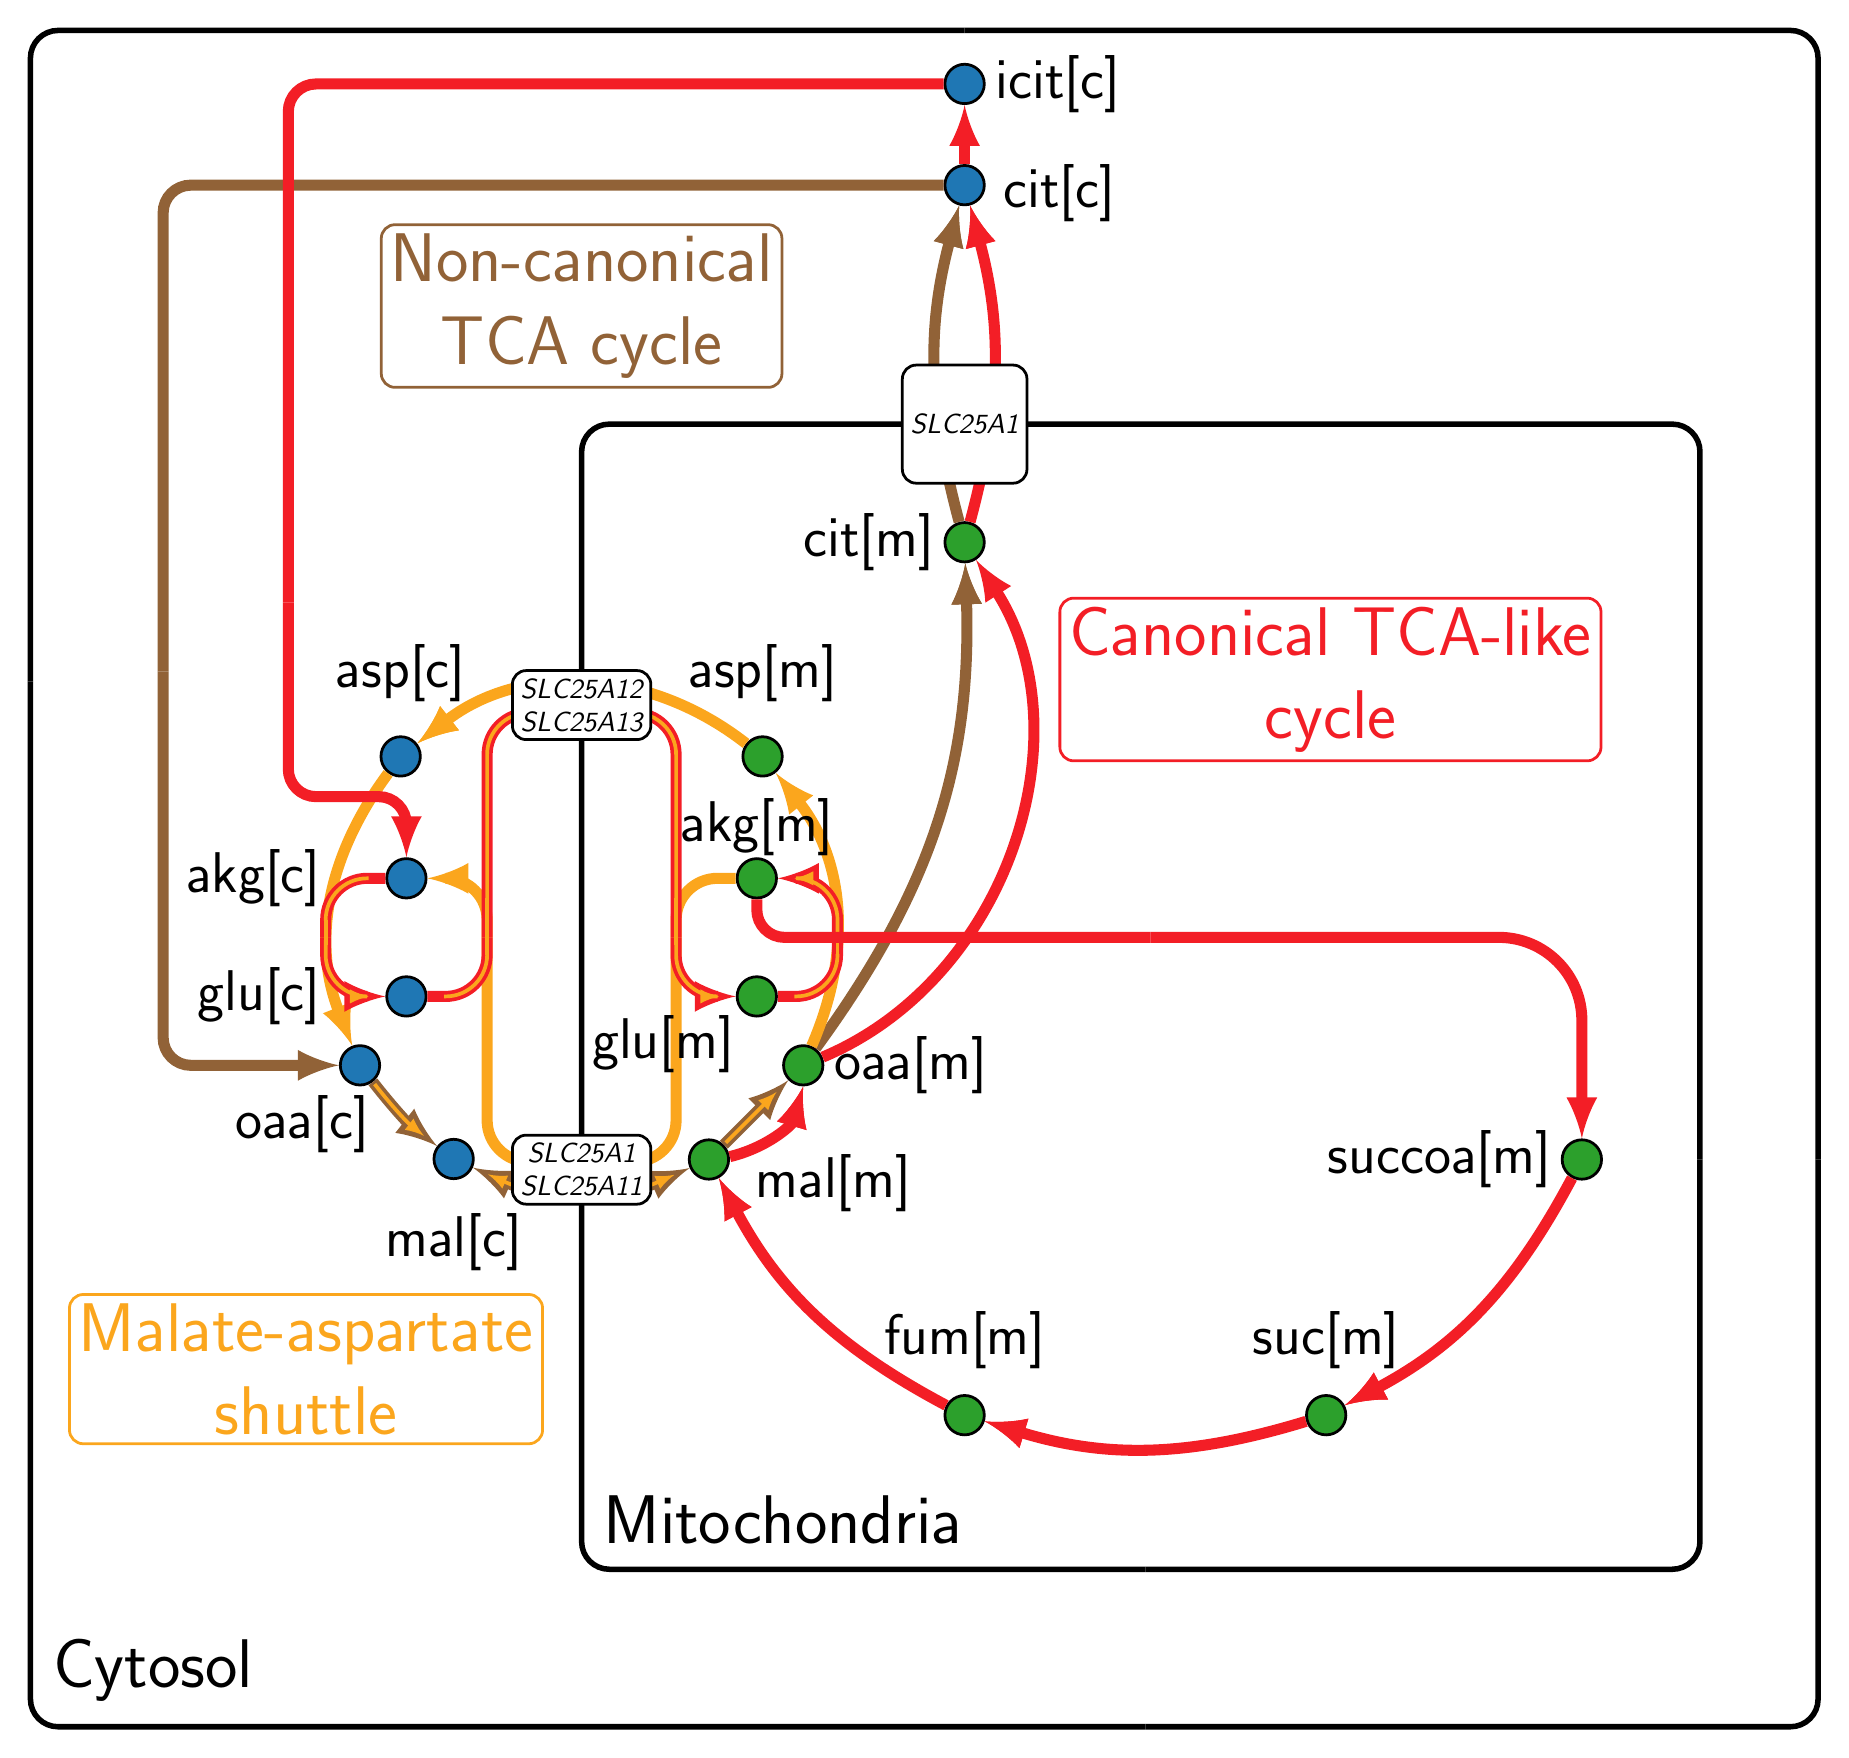
\begin{tikzpicture}[%
    >=latex,
    %-latex,
    decoration={%
        markings,mark=at position 1.0 with {\arrow{>}}
    },
    every node/.style={%
        font=\sffamily, %\itshape
        text=black,
        text centered,
        align=center
    },
]

    % Base position of main TCA circle
    \foreach \n in {1,2,...,16}{
        %\draw (\n*360/16+0: 6cm) node[node,fill=none,draw=black] (N\n) {\n};
        \draw (\n*360/16+0: 6cm) node[node,fill=none,draw=none] (N\n) {};
    }

    % Base position of malate-aspartate shuttle
    \foreach \m in {1,2,...,24}{
        %\draw (\m*360/24+0: 3.25cm) node[node,xshift=-7.160cm,yshift=+0.525cm,fill=none,draw=black] (M\m) {\m};
        \draw (\m*360/24+0: 3.25cm) node[node,xshift=-7.160cm,yshift=+0.525cm,fill=none,draw=none] (M\m) {};
    }


    % Base position for mitochondria compartment frame box
    \coordinate (B1) at ([xshift=-0.0cm]M6.center); % west
    \coordinate (B2) at ([yshift=1.5cm]N5.center); % north
    \coordinate (B3) at ([xshift=1.5cm]N15.center); % east
    \coordinate (B4) at ([yshift=-1.5cm]N12.center); % south
    
    \draw[-,line width=2pt,rounded corners=10pt] (B1) |- (B2);
    \draw[-,line width=2pt,rounded corners=10pt,name path=cit1] (B2) -| (B3);
    \draw[-,line width=2pt,rounded corners=10pt] (B1) |- (B4);
    \draw[-,line width=2pt,rounded corners=10pt] (B4) -| (B3);

    % Base position for cell frame box
    \coordinate (C1) at ([xshift=-7.0cm]M6.center); % west
    \coordinate (C2) at ([yshift=6.5cm]N5.center); % north
    \coordinate (C3) at ([xshift=3.0cm]N15.center); % east
    \coordinate (C4) at ([yshift=-3.5cm]N12.center); % south

    \draw[-,line width=2pt,rounded corners=10pt] (C1) |- (C2);
    \draw[-,line width=2pt,rounded corners=10pt] (C2) -| (C3);
    \draw[-,line width=2pt,rounded corners=10pt] (C1) |- (C4);
    \draw[-,line width=2pt,rounded corners=10pt] (C4) -| (C3);

    % TCA nodes
    \node[node,fill=mito] at (N9)  (malateM)      {};
    %\node[node,fill=mito] at (N7)  (oaaM)         {};
    \node[node,fill=mito] at (N5)  (citrateM)     {};
    %\node[node,fill=mito] at (N3)  (isocitrateM)  {};
    \node[node,fill=none,draw=none] at (N1)  (akgM)         {};
    \node[node,fill=mito] at (N15) (succinylcoaM) {};
    \node[node,fill=mito] at (N13) (succinateM)   {};
    \node[node,fill=mito] at (N11) (fumarateM)    {};

    % Malate-aspartate nodes
    \node[node,fill=mito] at (M3)  (aspartateM) {};
    \node[node,fill=none,draw=none] at (M6)  (aspTransporter) {};
    \node[node,fill=none,draw=none] at (M18) (malTransporter) {};
    \node[node,fill=cyto] at (M9)  (aspartateC) {};
    \node[node,fill=cyto] at (M14)  (oaaC) {};
    \node[node,fill=cyto] at (M16) (malateC) {};
    \node[node,fill=mito] at (M22) (oaaM2) {};

    \coordinate (C1) at ($(M12.center)!0.5!(M24.center)$);
    \node[node,fill=cyto,xshift=-0.6cm,yshift=+0.75cm] at ($(M12)!0.5!(C1.center)$) (akgC2) {};
    \node[node,fill=cyto,xshift=-0.6cm,yshift=-0.75cm] at ($(M12)!0.5!(C1.center)$) (glutamateC2) {};
    \node[node,fill=mito,xshift=+0.6cm,yshift=+0.75cm] at ($(M24)!0.5!(C1.center)$) (akgM2) {};
    \node[node,fill=mito,xshift=+0.6cm,yshift=-0.75cm] at ($(M24)!0.5!(C1.center)$) (glutamateM2) {};

    % Remaining cytoplasmic nodes
    \node[node,fill=cyto,above=4.0cm of N5] (citrateC) {};
    \node[node,fill=cyto,above=0.75cm of citrateC] (isocitrateC) {};
   
    % Grey TCA edges
    %\draw[-latex,postaction={decorate},line width=4pt,cgrey] (citrateM)          to [bend left=17] node [] {} (isocitrateM);
    %\draw[-latex,postaction={decorate},line width=4pt,cgrey,rounded corners=30pt] (isocitrateM) |- (akgM2);

    % Edges
    \draw[-latex,postaction={decorate},line width=4pt,efm2] (succinylcoaM)      to [bend left=17]  node [] {} (succinateM);
    \draw[-latex,postaction={decorate},line width=4pt,efm2] (succinateM)        to [bend left=17]  node [] {} (fumarateM);
    \draw[-latex,postaction={decorate},line width=4pt,efm2] (fumarateM)         to [bend left=17]  node [] {} (malateM);

    %\draw[double -latex=4pt colored by efm5 and efm2] (oaaM2)                   to [bend right=19] node [] {} (citrateM);
    \draw[-latex=4pt,postaction={decorate},line width=4pt,efm5] (oaaM2)         to [bend right=19] node [] {} (citrateM);
    \draw[-latex=4pt,postaction={decorate},line width=4pt,efm2] (oaaM2)         to [bend right=50] node [] {} (citrateM);
    \draw[double -latex=4pt colored by efm5 and efm4] (malateM)                 to [bend right=0]  node [] {} (oaaM2);
    \draw[-latex,postaction={decorate},line width=4pt,efm2] (malateM)           to [bend right=30] node [] {} (oaaM2.south);

    % Edges (malate-aspartate)
    \draw[double -latex=4pt colored by efm5 and efm4] (oaaC)                    to [bend right=7]  node [] {} (malateC);
    \draw[-latex,postaction={decorate},line width=4pt,efm4] (aspartateC)        to [bend right=29] node [] {} (oaaC);
    \draw[-latex,postaction={decorate},line width=4pt,efm4] (aspartateM)        to [bend right=38] node [] {} (aspartateC);
    \draw[double -latex2=4pt colored by efm5 and efm4] (malateC)                to [bend right=24] node [] {} (malateM);
    \draw[-latex,postaction={decorate},line width=4pt,efm4] (oaaM2)             to [bend right=31] node [] {} (aspartateM);

    % Edges (malate-aspartate inner)
    \draw[-,rounded corners=15pt,line width=4pt,efm4] ([xshift=-1.2cm]C1.center) |- ([yshift=+0.4cm]M18.center);
    \draw[-,rounded corners=15pt,line width=4pt,efm4] ([xshift=+1.2cm]C1.center) |- ([yshift=+0.4cm]M18.center);
    \draw[double -line=4pt colored by efm2 and efm4,rounded corners=15pt] (akgC2) -| (M12.center);
    \draw[double -latex=4pt colored by efm2 and efm4,rounded corners=15pt] (M12.center) |- (glutamateC2);
    \draw[latex-,rounded corners=15pt,line width=4pt,efm4] (akgC2) -| ([xshift=-1.2cm]C1.center);
    \draw[double -line=4pt colored by efm2 and efm4,rounded corners=15pt] (glutamateC2) -| ([xshift=-1.2cm]C1.center);
    \draw[-,rounded corners=15pt,line width=4pt,efm4] (akgM2) -| ([xshift=+1.2cm]C1.center);
    \draw[double -latex=4pt colored by efm2 and efm4,rounded corners=15pt] ([xshift=+1.2cm]C1.center) |- (glutamateM2);
    \draw[double -line=4pt colored by efm2 and efm4,rounded corners=15pt] ([xshift=-1.2cm]C1.center) |- ([yshift=-0.4cm]M6.center);
    \draw[double -line=4pt colored by efm2 and efm4,rounded corners=15pt] ([xshift=+1.2cm]C1.center) |- ([yshift=-0.4cm]M6.center);
    \draw[double -latex=4pt colored by efm2 and efm4,rounded corners=15pt] (M24.center) |- (akgM2);
    \draw[double -line=4pt colored by efm2 and efm4,rounded corners=15pt] (M24.center) |- (glutamateM2);

    % Hiding the extra red within inside malate-asparate shuttle
    \draw[line width=1.4pt, efm4] ([xshift=-1.2cm,yshift=-0.22cm]C1.center) to ([xshift=-1.2cm,yshift=+0.5cm]C1.center);
    \draw[line width=1.4pt, efm4] ([xshift=+1.2cm,yshift=-0.1cm]C1.center) to ([xshift=+1.2cm,yshift=+0.5cm]C1.center);

    \draw[line width=1.4pt, efm4] ([yshift=0.22cm]M12.center) to ([yshift=-0.1cm]M12.center);
    \draw[line width=1.4pt, efm4] ([yshift=0.1cm]M24.center) to ([yshift=-0.22cm]M24.center);

    % Edges (TCA cycle exiting mitochondrial citrate through malate-aspartate)
    %\draw[double -latex=4pt colored by efm5 and efm2] (citrateM)          to [bend right=0]  node [] {} (citrateC);
    \draw[-latex=4pt,postaction={decorate},line width=4pt,efm5] (citrateM)          to [bend left=15]   node [] {} (citrateC);
    \draw[-latex=4pt,postaction={decorate},line width=4pt,efm2] (citrateM)          to [bend right=15]  node [] {} (citrateC);
    \draw[-latex,line width=4pt,name path=cit2,draw=none] (citrateM)          to [bend right=0]  node [] {} (citrateC);
    \draw[latex-,line width=4pt,rounded corners=10pt,efm5] (oaaC) -| ([xshift=-2.5cm,yshift=5.0cm]oaaC.center);
    \draw[-,line width=4pt,rounded corners=10pt,efm5] (citrateC) -| ([xshift=-2.5cm,yshift=5.0cm]oaaC.center);
    \draw[-latex,line width=4pt,efm2] (citrateC)          to [bend right=0]  node [] {} (isocitrateC);
    \draw[-,line width=4pt,rounded corners=10pt,efm2] (isocitrateC) -| ([xshift=-1.5cm,yshift=5.0cm]glutamateC2.center);
    \node[] at ($(aspartateC)!0.33!(akgC2)$) (E1) {};
    \draw[-,line width=4pt,rounded corners=10pt,efm2] ([xshift=-1.5cm,yshift=5.0cm]glutamateC2.center) |- ([xshift=-0.5cm]E1.center) ;
    \draw[-latex,line width=4pt,rounded corners=10pt,efm2] ([xshift=-0.5cm]E1.center)  -| (akgC2.north);

    % Edges (TCA)
    \node[] at ($(akgM2)!0.5!(glutamateM2)$) (D1) {};
    \draw[-,line width=4pt,efm2,rounded corners=10pt] (akgM2.south) |- ([xshift=5.0cm]D1.center);
    \draw[-latex,line width=4pt,efm2,rounded corners=30pt] ([xshift=5.0cm]D1.center) -| (succinylcoaM.north);
    
    % Transporters
    \fill [name intersections={of=cit1 and cit2}] (intersection-1) circle (0pt) node[nodeT2,font=\it] () {SLC25A1};
    \node[nodeT1,font=\it] at ([yshift=+0.3cm]M18.center) {SLC25A1\\SLC25A11};
    \node[nodeT1,font=\it] at ([yshift=-0.3cm]M6.center) {SLC25A12\\SLC25A13};

    % Metabolite labels
    \node[font=\huge,right=0.1cm of isocitrateC,xshift=-0.1cm] () {icit[c]};
    \node[font=\huge,right=0.1cm of citrateC,yshift=-0.1cm] () {cit[c]};
    \node[font=\huge,left=0.1cm of citrateM,xshift=+0.1cm] () {cit[m]};
    \node[font=\huge,left=0.1cm of succinylcoaM,xshift=+0.1cm] () {succoa[m]};
    \node[font=\huge,above=0.1cm of succinateM,xshift=+0.0cm,yshift=+0.1cm] () {suc[m]};
    \node[font=\huge,above=0.1cm of fumarateM,yshift=+0.1cm] () {fum[m]};
    \node[font=\huge,above=0.1cm of aspartateC,yshift=+0.2cm] () {asp[c]};
    \node[font=\huge,above=0.1cm of aspartateM,yshift=+0.2cm] () {asp[m]};
    \node[font=\huge,right=0.1cm of oaaM2,xshift=-0.1cm] () {oaa[m]};
    \node[font=\huge,below left=0.1cm of oaaC,xshift=+0.5cm] () {oaa[c]};
    \node[font=\huge,right=0.1cm of malateM,xshift=+0.1cm,yshift=-0.3cm] () {mal[m]};
    \node[font=\huge,below=0.1cm of malateC,yshift=-0.2cm] () {mal[c]};

    \node[font=\huge,left=0.7cm of glutamateC2] () {glu[c]};
    %\node[font=\huge,right=1.0cm of glutamateM2,xshift=+0.0cm,yshift=0.0cm] () {glu[m]};
    \node[font=\huge,left=0.1cm of glutamateM2,xshift=+0.2cm,yshift=-0.6cm] () {glu[m]};
    \node[font=\huge,left=0.7cm of akgC2,xshift=-0.0cm] () {akg[c]};
    \node[font=\huge,above=0.1cm of akgM2,yshift=-0.2cm] () {akg[m]};

    % Pathway labels
    \node[rectangle,rounded corners=5pt,draw,line width=1pt,below=1.0cm of M18,align=center,font=\Huge,xshift=-3.5cm,efm4] () {Malate-aspartate\\shuttle};
    \node[rectangle,rounded corners=5pt,draw,line width=1pt,above=3.45cm of M6, align=center,font=\Huge,efm5] () {Non-canonical\\TCA cycle};
    \node[rectangle,rounded corners=5pt,draw,line width=1pt,xshift=2.35cm,yshift=+3.8cm,align=center,font=\Huge,efm2] () {Canonical TCA-like\\cycle};
    %\node[rectangle,rounded corners=5pt,draw,line width=1pt,xshift=4.65cm,yshift=+4.0cm,align=center,font=\Huge,cgrey] () {Canonical\\TCA cycle\\steps};

    % Compartment labels
    \node[align=center,font=\Huge,above=0.2cm of B4,xshift=-4.6cm] () {Mitochondria};
    \node[align=center,font=\Huge,above=0.2cm of C4,xshift=-12.6cm] () {Cytosol};

\end{tikzpicture}

\end{document}

